\section[Theorie]{Theorie\footcite{man:v103}}
Die Spannung $\sigma$ ist die Kraft pro Flächeneinheit, die auf einen gedehnten Körper wirkt.
Das Elastizitätsmodul $E$ ist eine Kenngröße für die Elastische Ausdehnung von Materialien. % Die Reihenfolge ist nicht so geil...
Im Hookeschen Gesetz verbindet $E$ die elastische Spannung $\sigma$ mit der Ausdehnung entlang einer Fläche
\begin{align}
    \sigma = E \frac{\Delta L}{L}.
    \label{eq:Hook_Gesetz}
\end{align}
\begin{figure}[H]
    \centering
    \includegraphics[width=0.6\textwidth]{Abbildungen/Längenausdehnung.png}
    \caption{Dehnung eines Stabförmigen Materials in der Länge \cite{man:v103}.}
    \label{fig:laengenausdehnung}
\end{figure}
\noindent
Dieser Lineare Zusammenhang, ist nur bei sehr kleinen Auslenkungen gültig.
Bei größeren Dehnungen beginnt die plastische Verformung, die in diesem Versuch nicht betrachtet werden soll.
Mit den geeigneten Messvorrichtungen, die auch sehr kleine Auslenkungen eines Stabes messen kann, 
könnte $E$ direkt gemessen werden.
So eine Vorrichtung ist hier aber nicht vorhanden. 
Die Elastizität wird deshalb in der Biegung des Stabes beobachtet, da hier auch kleinere Kräfte für größere Auslenkungen genügen.

Um die Auslenkung des Stabes zu berechnen muss die Stärke des inneren Drehmoments $M_\sigma$ berechnet werden, 
die dem äußeren Drehmoment entgegenwirkt.
Bei der Biegung des Stabs wird die obere Hälfte gestreckt und die untere Hälfte gestaucht.
In der Mitte gibt es eine neutrale Faser, die weder gestreckt noch gestaucht wird.
Diese neutrale Faser liegt in den Koordinatensystemen bei $y = 0$ 
Das Drehmoment, das der Verbiegung entgegenwirkt wird mit 
\begin{align}
    M_\sigma = \int_{Q}^{} y \sigma(y) \,\diff q 
    \label{eq:inneres_Moment_int}
\end{align}
berechnet.
\begin{figure}
    \centering
    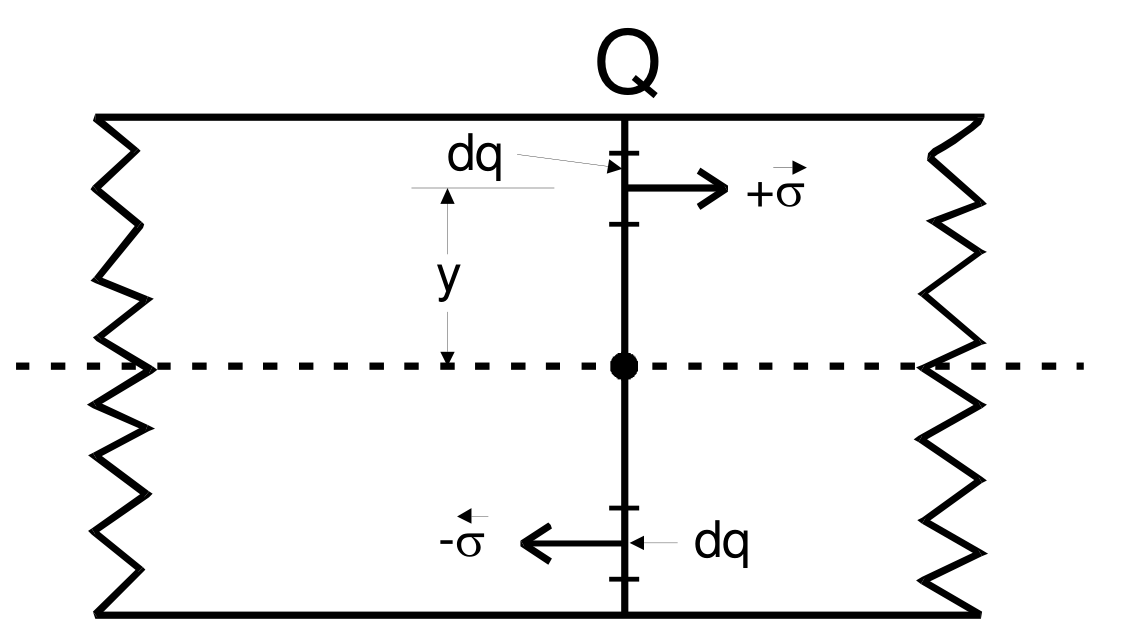
\includegraphics[width = 0.5\textwidth]{Abbildungen/Biegungsintegral.png}
    \caption{Skizze zur Berechnung des Flächenträgheitsmomentes \cite{man:v103}}
    \label{fig:Biegungsintegral}
\end{figure}
Hier wird ein Integral über den Querschnitt der Stange berechnet (vgl. Abb \ref{fig:Biegungsintegral}).
In der Näherung für kleine Winkel gilt für $\sigma(y)$
\begin{align*}
    \sigma(y) = E \frac{y}{R} .
\end{align*}
Mit der Auslenkung $D(x)$ des Stabs kann eine Näherung für den Krümmungsradius $R$ gefunden werden.
\begin{align*}
    \frac{1}{R} &\simeq  \frac{\diff^2 D}{\diff x^2} & &\text{wenn} & \left(\frac{\diff D}{\diff x}\right)^2 << 1 
\end{align*}
Schließlich wird für die einseitige Biegung des Stabes das äußere Drehmoment $M_F = F(L - x)$ mit dem Inneren Drehmoment gleichgesetzt.
Nach den Näherungen für $\sigma(y)$ ergibt sich
\begin{align}
    M_\sigma = E \, \frac{\diff^2 D}{\diff x^2} \int_{Q} y^2 \,\diff q = F (L - x) = M_F  . % Man kann hier auch einfach I einsetzen in der Auswertung.
    \label{eq:Momentengleichung_einseitig}
\end{align}
Der Therm 
\begin{align}
    I := \int_{Q} y^2 \,\diff q
\end{align} 
wird als Flächenträgheitsmoment bezeichnet.
In diesem Versuch gibt es eine runde und eine Rechteckige Stange.
Laut \cite{uni_siegen} ergeben sich für einen quadratischen Stab mit der Seitenlänge $a$ und einen runden Stab mit dem Radius $r$ folgende Flächenträgheitsmomente
\begin{align}
    I_\text{rechteckig} &= \frac{a^4}{12} & I_\text{rund} &= \frac{\pi r^4}{4}
    \label{eq:Flachentragheitsmomente}
\end{align}
%
Durch Integration über D ergibt sich für die Auslenkung die Formel
\begin{align}
    D(x) = \frac{F}{2 E I} \left(L x^2 - \frac{x^3}{3} \right)
    \label{eq:D_x_einseitig}
\end{align}
bei der einseitigen Einspannung.
Wenn der Stab an beiden Seiten aufgehängt wird ergibt sich für die Auslenkung von x für
$0 \leq x \leq L/2$
\begin{align}
    D(x) = \frac{F}{48 E I} \left(3 L^2- 4 x^3\right).
    \label{eq:D_x_links}
\end{align}
Für die Auslenkung auf der Rechten Seite ($L/2 \leq x \leq L $) folgt
\begin{align}
    D(x) = \frac{F}{48 E I} \left(4x^3 - 12L x^2 + 9L^2 x - L^3 \right). 
    \label{eq:D_x_beidseitig_links}
\end{align}